\subsection{Vérifications préliminaires}

Avant d'exploiter les résultats de température issus des simulations, deux vérifications préliminaires ont été menées afin de s'assurer de la cohérence physique du montage numérique.

La première concerne le profil de puissance imposé dans le combustible. La puissance volumique déposée devant suivre un profil axial en cosinus, représentatif de la distribution de puissance neutronique le long d'un crayon, le profil de température visible sur la Figure \ref{fig:profil} montre une bonne adéquation des résultats de la simulation avec les attentes.

\begin{figure}[H]
\centering
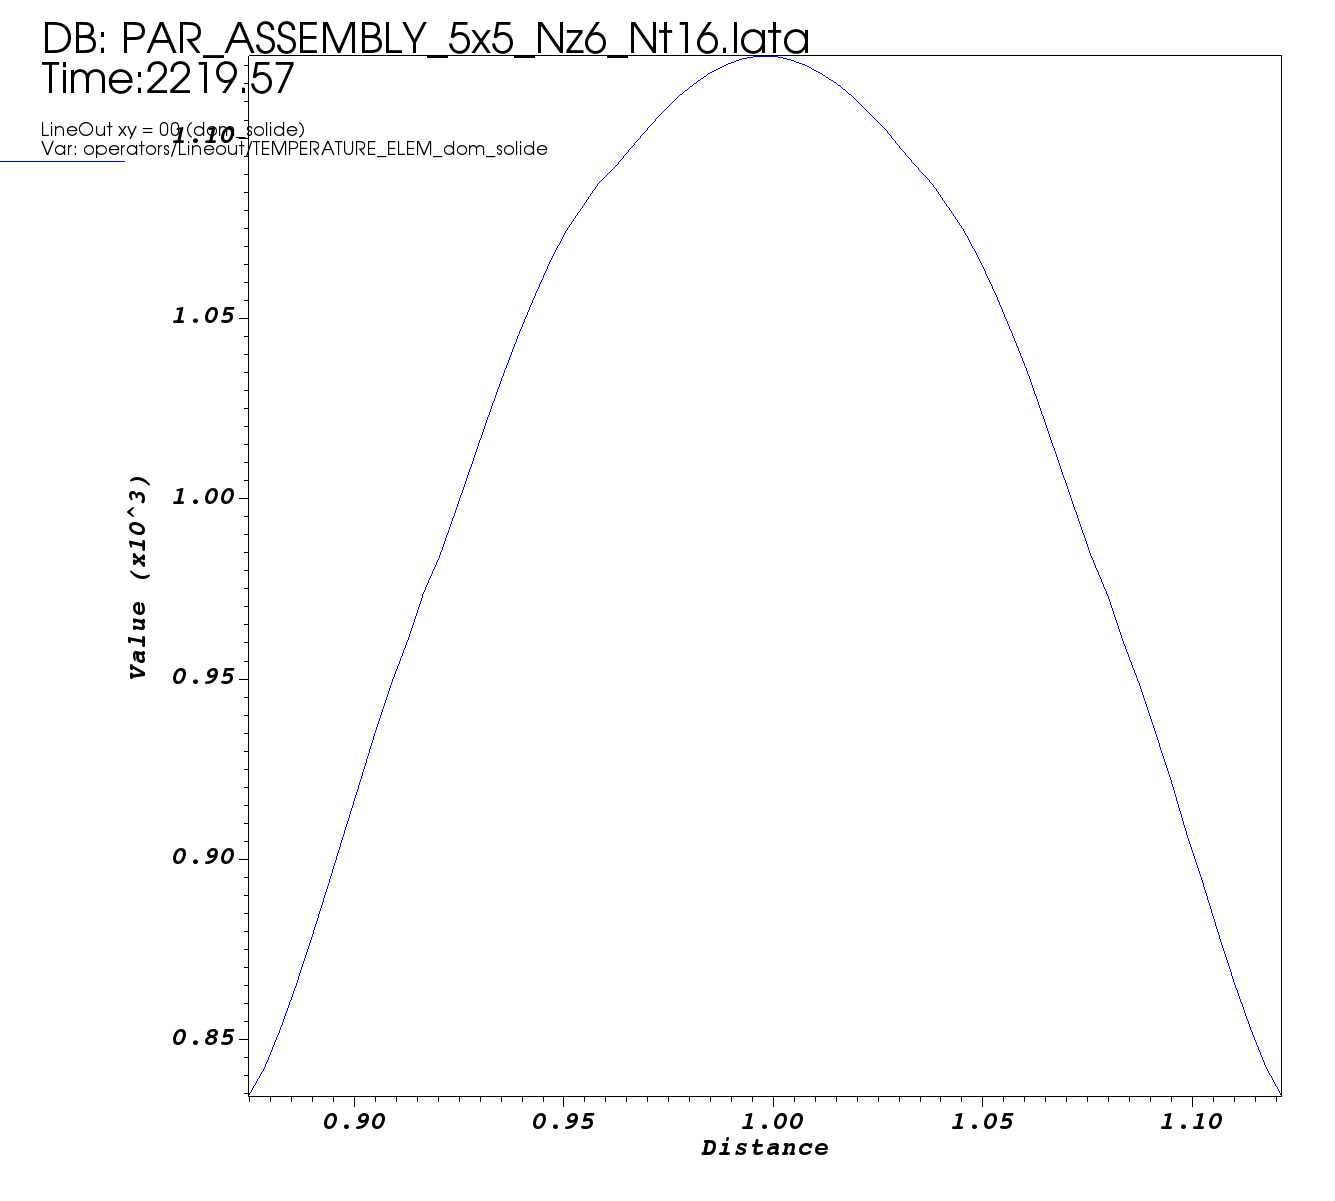
\includegraphics[width=0.6\linewidth]{PICTURES/c5couplage/lineout.png}
\caption{Profil axial de température au centre du crayon central.}
\label{fig:profil}
\end{figure}
La seconde vérification porte sur la conservation globale de l'énergie au sein du système. En régime stationnaire, la puissance totale déposée dans le combustible doit être intégralement évacuée par les mécanismes de transfert thermique du domaine, à savoir la conduction vers la paroi et la convection au sein du fluide caloporteur. Le bilan global de puissance s'écrit ainsi :

\begin{equation}
    P_{\mathrm{volumique}} = P_{\mathrm{sortant}}
    \label{eq:bilan_puissance}
\end{equation}

où $P_{\mathrm{déposée}}$ désigne la puissance volumique totale injectée dans le combustible, et $P_{\mathrm{sortant}} = P_{\mathrm{rad}} + P_{\mathrm{diffusion}}$ les puissances évacuées par les parois du domaine. Cette égalité a été vérifiée sur la plupart des cas étudiés, avec un écart relatif entre la dizaine de $pcm$ au $\%$, confirmant même dans le pire des cas la cohérence du bilan thermique global de la simulation.

\subsection{Conséquence de l'hypothèse de radiosité uniforme}
\begin{figure}[H]
\centering
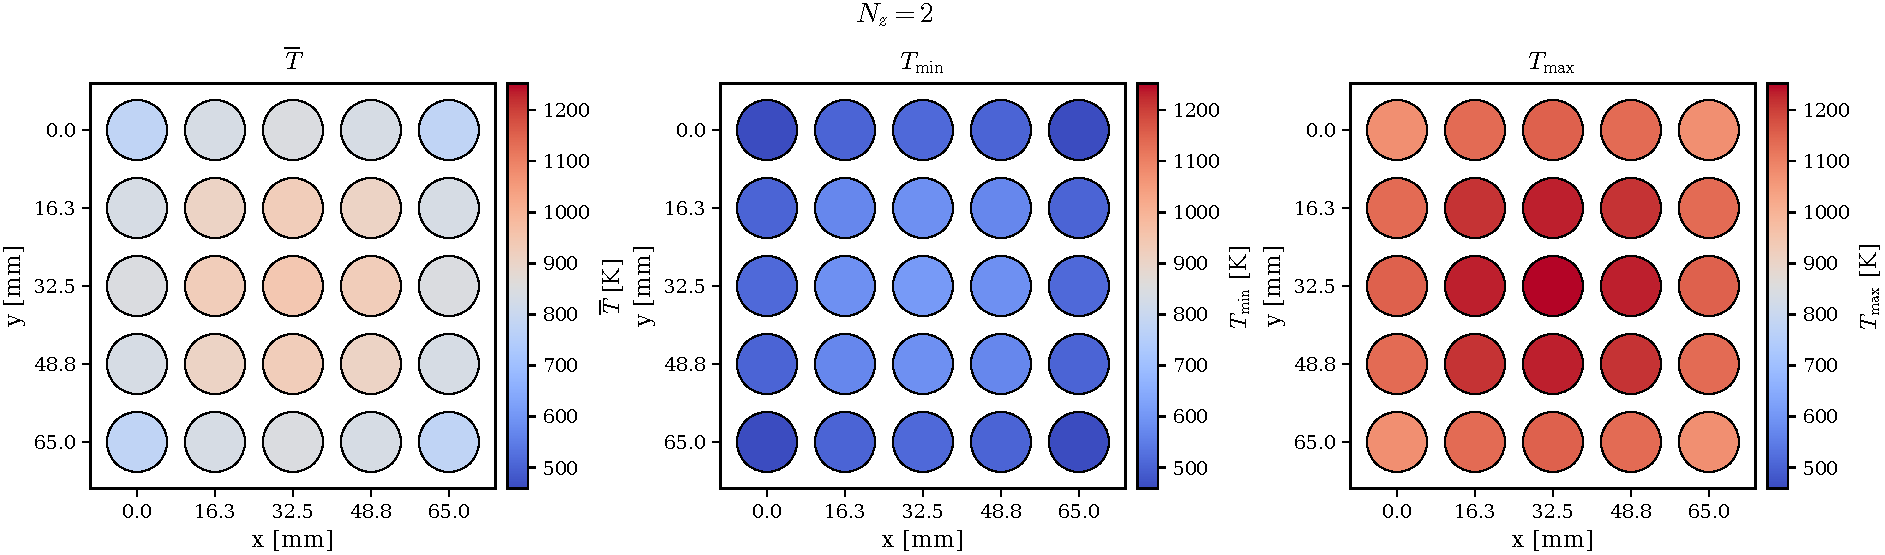
\includegraphics[width=0.8\linewidth]{PICTURES/c5couplage/T925/assembly_2.pdf}
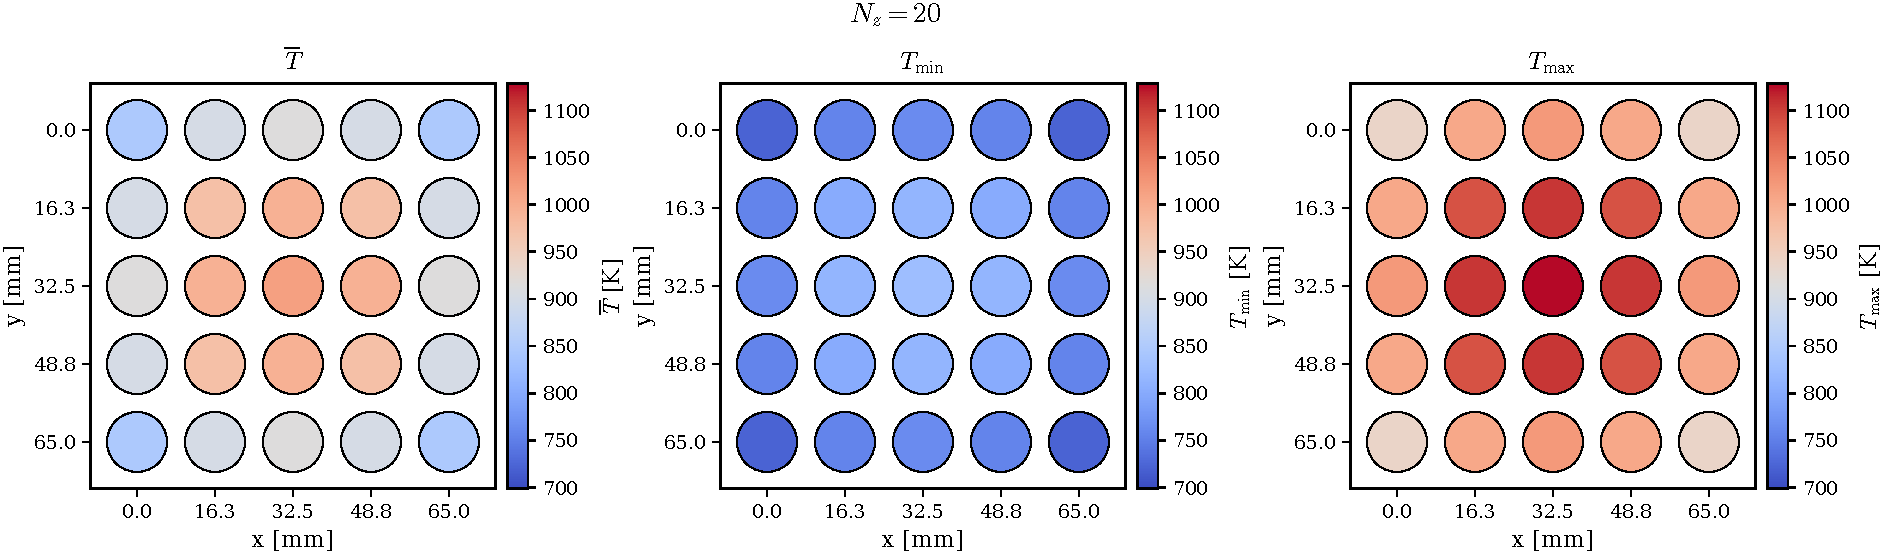
\includegraphics[width=0.8\linewidth]{PICTURES/c5couplage/T925/assembly_20.pdf}
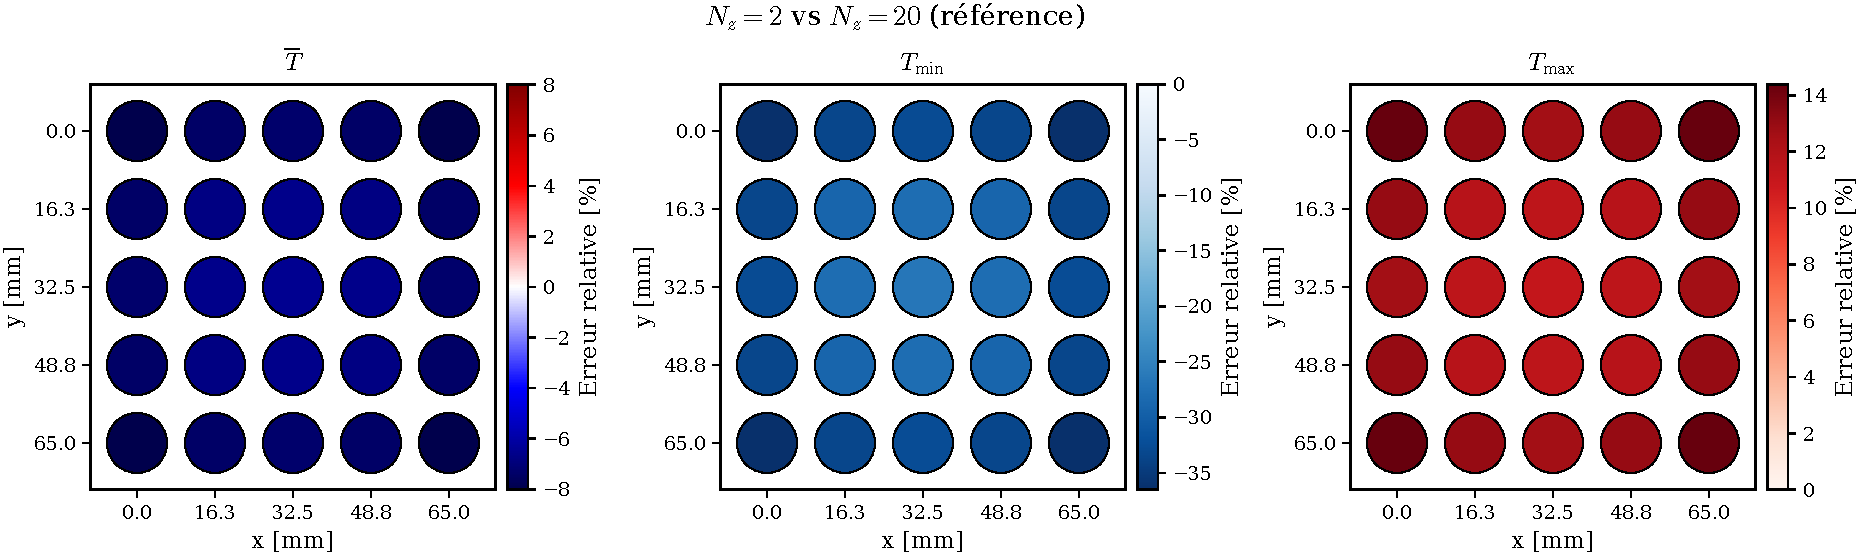
\includegraphics[width=0.8\linewidth]{PICTURES/c5couplage/T925/assembly_diff_2_vs_20.pdf}

 \caption{Températures minimum, maximum et moyenne dans le cas $\overline{T}=925.7$~K}
 \label{fig:temperature3MW}
\end{figure}



\begin{figure}[H]
\centering
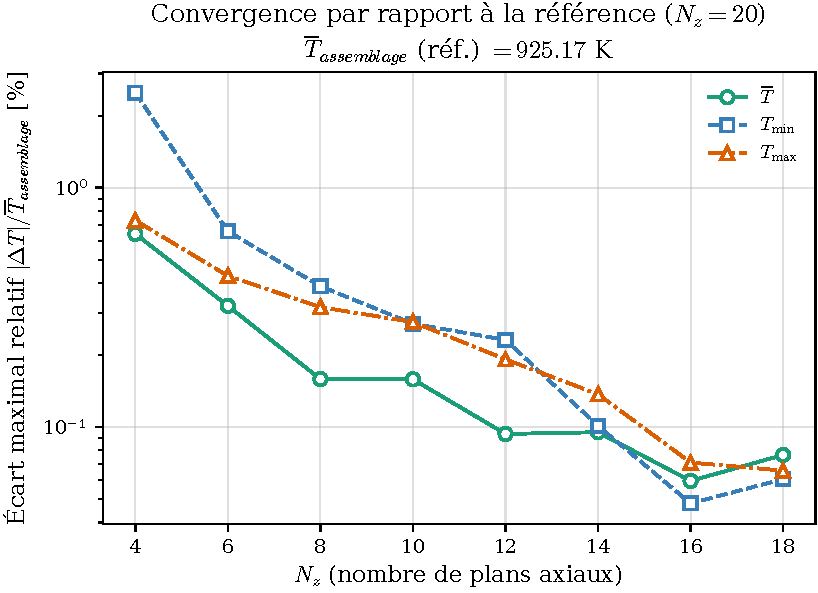
\includegraphics[width=0.7\linewidth]{PICTURES/c5couplage/T925/convergence_relative_vs_20.pdf}

 \caption{Convergence relative des températures dans le cas $\overline{T}=925.7$~K}
 \label{fig:convergence3MW}
\end{figure}




\begin{figure}[H]
\centering
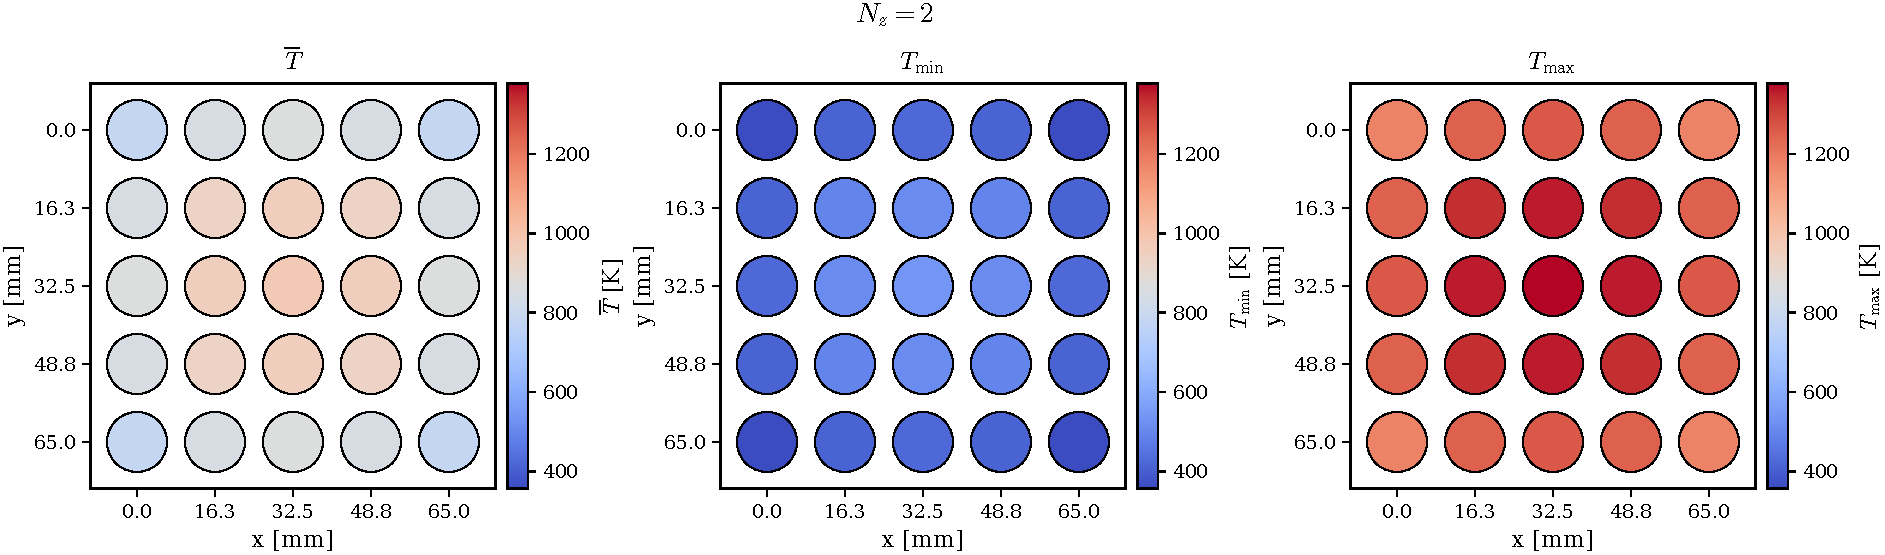
\includegraphics[width=0.8\linewidth]{PICTURES/c5couplage/T1000/assembly_2.pdf}
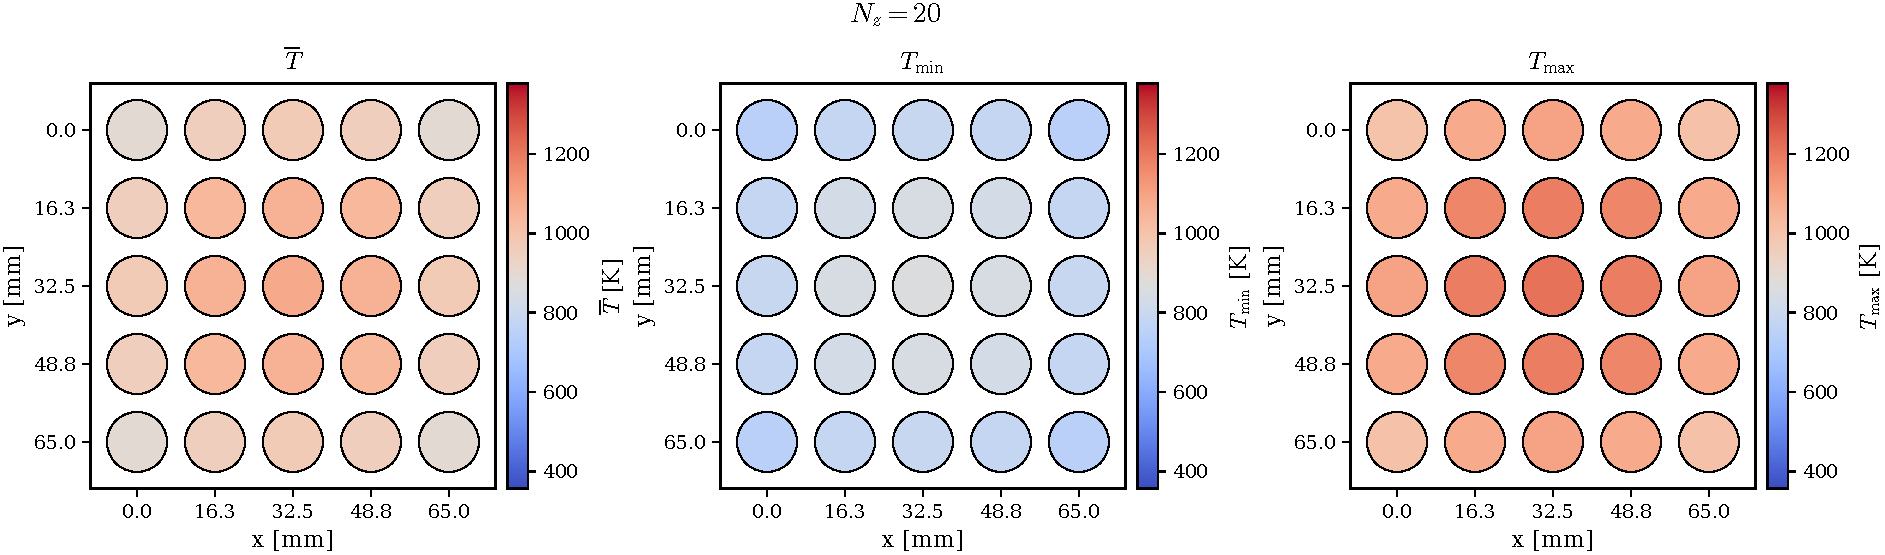
\includegraphics[width=0.8\linewidth]{PICTURES/c5couplage/T1000/assembly_20.pdf}
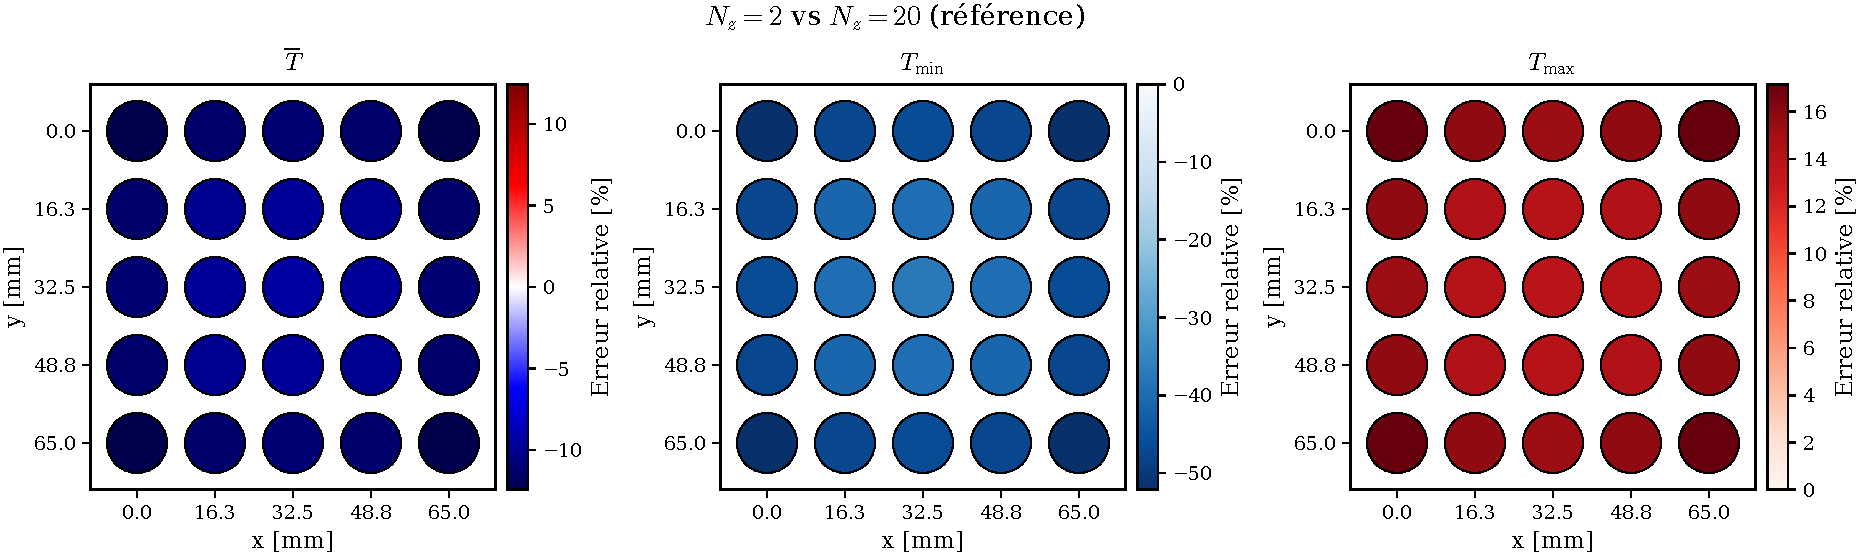
\includegraphics[width=0.8\linewidth]{PICTURES/c5couplage/T1000/assembly_diff_2_vs_20.pdf}

 \caption{Températures minimum, maximum et moyenne dans le cas $\overline{T}=981.4$~K}
 \label{fig:temperature4MW}
\end{figure}



\begin{figure}[H]
\centering
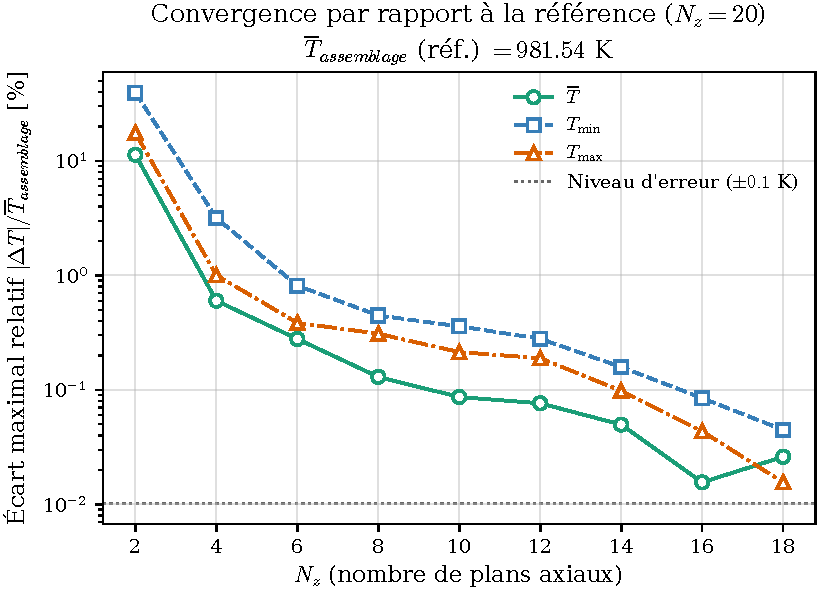
\includegraphics[width=0.7\linewidth]{PICTURES/c5couplage/T1000/convergence_relative_vs_20.pdf}

 \caption{Convergence relative des températures dans le cas $\overline{T}=981.4$~K}
 \label{fig:convergence4MW}
\end{figure}


\subsection{Etude de l'écart entre le point chaud et la température moyenne}
Le Tableau~\ref{tab:tmoy_tmax} rassemble, pour les trois niveaux de puissance étudiés, la température moyenne $T_{\mathrm{moy}}$ et la température maximale $T_{\mathrm{max}}$ obtenues sur le crayon central. On observe que l'écart entre $T_{\mathrm{max}}$ et $T_{\mathrm{moy}}$ croît avec le niveau de puissance déposée, aussi bien en valeur absolue qu'en proportion de la température moyenne. L'intérêt de ce résultat ne réside cependant pas dans ces trois seules valeurs, dont le nombre reste insuffisant pour en tirer une conclusion générale, mais dans la démarche qu'elles illustrent : la capacité à quantifier, à partir d'une simulation CFD 3D complète, l'écart entre température moyenne et température de point chaud pour une configuration donnée. Une telle relation, une fois établie sur un nombre suffisant de cas, ouvrirait la voie à l'estimation de la température de point chaud d'un système à partir de sa seule température moyenne, cette dernière étant directement accessible par des modèles à zones plus simples et bien moins coûteux en temps de calcul que la simulation CFD 3D complète.

\begin{table}[H]
\centering
\begin{tabular}{ccccc}
\toprule
Cas & Puissance volumique~[$\mathrm{MW/m^3}$] & $T_{\mathrm{moy}}$~[K] & $T_{\mathrm{max}}$~[K] & Écart relatif $\frac{T_{\mathrm{max}} - T_{\mathrm{moy}}}{T_{\mathrm{moy}}}$ \\
\midrule
1 & $3$  & $925{,}2$ & $1127$ & \red{...} \\
2 & $4$  & $981{,}5$ & $1211$ & \red{...} \\
3 & $45$ & $1817$    & $2475$ & \red{...} \\
\bottomrule
\end{tabular}
\caption{Températures moyenne et maximale du crayon central pour les trois niveaux de puissance étudiés.}
\label{tab:tmoy_tmax}
\end{table}



\subsection{Conclusion}